\documentclass[11pt]{article}
\usepackage[a4paper,margin=2.4cm]{geometry}
\usepackage{amsmath,amssymb}
\usepackage{graphicx}
\usepackage{booktabs}
\usepackage[authoryear,round]{natbib}
\usepackage{microtype}
\usepackage[colorlinks=true,linkcolor=blue!50!black,citecolor=blue!50!black,urlcolor=blue!50!black]{hyperref}
\usepackage{xcolor}
\usepackage{url}\urlstyle{same}

\newcommand{\aL}{a_\Lambda}
\newcommand{\unit}[1]{\,\mathrm{#1}}
\newcommand{\aunit}{\times10^{-10}\unit{m\,s^{-2}}}

\title{\Large\textbf{Rings of Presence:\\ one balance rule for gravitational boundaries,\\ and the galactic acceleration scale as $c^2\sqrt{\Lambda/3}\,/\,2\pi$}}
\author{Hassan Anwar\\[2pt]
\small Independent researcher, Pakistan\\
\small \href{mailto:hassanalgo12@gmail.com}{hassanalgo12@gmail.com}}
\date{October 2026}

\begin{document}
\maketitle

\begin{abstract}
\noindent
We describe weak-field gravity with one dimensionless field, the \emph{presence} $P=\sum_i G E_i/(c^4 r_i)=-\Phi/c^2$, whose value, gradient and Hessian give clock rates, accelerations and tides. This is a reorganisation of weak-field general relativity, not a modification, and it reproduces the standard tests by construction. We use it for two results.
(i) The Hill radius, the Jacobi tidal radius, the L1 distance and the largest turnaround radius allowed by a cosmological constant all follow from one balance condition, $r^3=Gm/S$, where $S$ is the stretching rate of the environment, ending in $S=\Lambda c^2/3$ for empty space. The outermost moons of six planets lie within $0.46\,r$, 107 of 111 satellites of the Milky Way and M31 lie inside their hosts' radii, and the zero-velocity radii of the Local Group and Virgo lie inside their $\Lambda$ limits.
(ii) Treating empty space as the outermost host of every system, we propose that the acceleration scale of the radial acceleration relation is $a_0=\aL/k$, with $\aL=c^2\sqrt{\Lambda/3}$ and $k$ the total presence of a point source inside a ring divided by its presence at the edge, in units of the ring's size. This integral equals $2\pi$ for both planar and spherical rings, which gives a reason for the long-noted coincidence $2\pi a_0\approx c^2(\Lambda/3)^{1/2}$ and a parameter-free prediction, $a_0=0.86\aunit$ (Planck) or $0.94\aunit$ (SH0ES).
Sixteen gas-rich SPARC galaxies give $0.82^{+0.22}_{-0.17}\aunit$, in agreement. The full sample of 164 galaxies gives $1.14\pm0.08\aunit$ at the fiducial stellar mass-to-light ratio $\Upsilon_{\rm disk}=0.5$ and matches the prediction for $\Upsilon_{\rm disk}\approx0.6$. Per-galaxy $a_0$ shows no dependence on size, distance, surface brightness, rotation speed, gas fraction or bulge fraction, as the scale-free integral requires. Forty-one disks at $z=0.65$--$2.45$ show no rise of $a_0$ with redshift, though they cannot yet exclude $a_0\propto H(z)$. We state which observations can confirm or exclude the proposal.
\end{abstract}

\section{Introduction}

Rotationally supported galaxies obey a tight radial acceleration relation (RAR) between the observed centripetal acceleration $g_{\rm obs}$ and the acceleration $g_{\rm bar}$ produced by their baryons \citep{McGaugh2016,Lelli2017}. The relation is Newtonian at high acceleration and departs from it below a scale $a_0\approx1.2\aunit$ that appears to be the same in every galaxy \citep{Li2018}. Whether the RAR reflects modified dynamics \citep{Milgrom1983,FamaeyMcGaugh2012} or emerges from galaxy formation with cold dark matter \citep{KellerWadsley2017,Ludlow2017}, the numerical value of $a_0$ is an empirical input. It has long been noted that $2\pi a_0\approx cH_0\approx c^2(\Lambda/3)^{1/2}$ \citep{Milgrom1983,Milgrom1999,Milgrom2016}, but the factor $2\pi$ has no accepted derivation.

A second link between local dynamics and $\Lambda$ is well understood: a cosmological constant sets a largest possible turnaround radius, $R_\Lambda=(3GM/\Lambda c^2)^{1/3}$, for any bound structure \citep{PavlidouTomaras2014}.

This paper organises weak-field gravity around one scalar, the \emph{presence}, and uses it for two results. We are explicit about which parts are new. Sections~\ref{sec:presence} and \ref{sec:rings} restate known physics in one language: the presence is the Newtonian potential divided by $-c^2$, and the boundary rule unifies results that are individually standard. Their value is that one number describes every scale, from a moon to the edge of a galaxy group, and that empty space appears as the outermost environment of every system. Section~\ref{sec:a0} contains the one proposal that goes beyond current physics: a derivation of the factor $2\pi$ in the $a_0$--$\Lambda$ relation from a presence integral, with no adjustable parameter. We test it on the SPARC rotation curves \citep{Lelli2016} and on disks at $z\approx1$--2.4 \citep{Price2021}. Section~\ref{sec:discussion} discusses the stellar mass-to-light systematic, which currently limits the test, and the observations that can decide. Every number in the paper is produced by public scripts.

\section{Presence: weak-field gravity as one scalar}
\label{sec:presence}

For sources with energies $E_i$ (for matter at rest $E_i=m_ic^2$) at distances $r_i$,
\begin{equation}
P(\mathbf{x})=\sum_i\frac{G E_i}{c^4\,r_i}=-\frac{\Phi(\mathbf{x})}{c^2},
\label{eq:presence}
\end{equation}
where $\Phi$ is the Newtonian potential. $P$ is dimensionless and small: about $7\times10^{-10}$ at Earth's surface, $10^{-8}$ from the Sun at 1\,au and $2\times10^{-6}$ at the solar surface. In the isotropic weak-field metric $ds^2=-(1-2P)\,c^2dt^2+(1+2P)\,d\mathbf{x}^2$, three readings of the same field carry most of weak-field gravity:
\begin{itemize}
\item its \emph{value} sets clock rates, $d\tau/dt\simeq1-P-v^2/2c^2$;
\item its \emph{gradient} is the acceleration, $\mathbf{g}=c^2\nabla P$;
\item its \emph{Hessian} is the tidal tensor, $T_{ij}=c^2\,\partial_i\partial_jP$, of magnitude $2GMd/D^3$ across a body of size $d$ at distance $D$ from a mass $M$.
\end{itemize}

\paragraph{Thought experiment: the room inside a shell.} Place a laboratory at the centre of a large, uniform shell of matter. The shell raises $P$ everywhere inside by the same amount, so every clock in the room slows equally and nothing is pulled anywhere. No local experiment can detect the shell. Only differences, slopes and changes of slope of $P$ are observable. This is why the presence of the whole Universe, of order unity at every point, has no local effect.

Light deflection, perihelion advance and radar delay follow from the metric as in general relativity, and orbital decay by gravitational radiation from the Peters--Mathews luminosity. Table~\ref{tab:standard} lists the values we recover. They agree because the description is equivalent to weak-field general relativity; we list them only to show that the bookkeeping is right.

\begin{table}[t]
\centering
\caption{Standard tests recovered by the presence description (identical to general relativity by construction). Measurements: GPS, \citet{Ashby2003}; deflection and perihelion, \citet{Will2014}; PSR B1913+16, \citet{WeisbergHuang2016}; millimetre-scale redshift, \citet{Bothwell2022}; lunar laser ranging, \citet{Muller2023}; light deflected by light, \citet{Tolman1931}; tides, the S2/M2 equilibrium ratio.}
\label{tab:standard}
\small
\begin{tabular}{@{}llll@{}}
\toprule
Test & Reading of $P$ & Computed & Measured / known \\
\midrule
GPS satellite clock offset & value, with $v^2/2c^2$ & $+38.51\unit{\mu s\,d^{-1}}$ & $+38.58\unit{\mu s\,d^{-1}}$ (built in)\\
Light deflection, solar limb & $\alpha=4P$ & $1.751''$ & $1.75''$\\
Perihelion advance, Mercury & $6\pi P$ per orbit & $42.98''\,{\rm cy}^{-1}$ & $43''\,{\rm cy}^{-1}$\\
Orbital decay, PSR B1913+16 & Peters--Mathews & $1.0001\times$ GR & $(0.9983\pm0.0016)\times$ GR\\
Redshift across 1\,mm & value & $1.09\times10^{-19}$ & $(0.98\pm0.23)\times10^{-19}$\\
Nordtvedt $\eta$, Earth--Moon & gradient & $0$ & $(-0.2\pm1.1)\times10^{-4}$\\
Light deflected by light & $\alpha=8GE/c^4b$ head-on & $0$ side by side & same \\
Solar/lunar tide ratio & Hessian & $0.46$ & $0.46$\\
\bottomrule
\end{tabular}
\end{table}

\section{One balance rule for gravitational boundaries}
\label{sec:rings}

\subsection{The rule}

A body of mass $m$ sits in an environment whose tidal field, in the frame moving with the body, stretches nearby test particles at a rate $S$. Here $S$ is the largest eigenvalue of the effective tidal tensor, including the centrifugal term when the frame rotates. Along that direction a test particle at distance $r$ feels $-Gm/r^2+S\,r$. The body controls the region where its own pull wins, which ends at
\begin{equation}
r_{\rm own}^3=\frac{G\,m}{S}.
\label{eq:own}
\end{equation}
The environment fixes $S$:
\begin{itemize}
\item \textbf{Point-mass host} $M$ at distance $D$, circular orbit: $S=\Omega^2-\partial^2\Phi/\partial D^2=3GM/D^3$. This gives $r_{\rm own}=D\,(m/3M)^{1/3}$, the Hill radius and the distance to L1 and L2 \citep{MurrayDermott1999}.
\item \textbf{Extended host} with a flat rotation curve $V_c$: $S=2V_c^2/D^2$, which gives the Jacobi tidal radius \citep{King1962}.
\item \textbf{Empty space}: the background acceleration $+\tfrac13\Lambda c^2 r$ is isotropic and the same everywhere, so $S=\Lambda c^2/3$. This gives $r_{\rm own}=R_\Lambda=(3Gm/\Lambda c^2)^{1/3}$, the zero-gravity radius and largest turnaround radius \citep{PavlidouTomaras2014}.
\end{itemize}
For comparable masses we use the volume-equivalent Roche-lobe radius \citep{Eggleton1983}, which for small mass ratios is 0.71 of the L1 distance. Equation~(\ref{eq:own}) contains no new physics. What it adds is a single quantity, $S$, that characterises the environment of any bound system, with empty space as the final environment.

\paragraph{Thought experiment: pebbles at the edge.} Release pebbles at increasing distances from the Moon. Close in they fall back to the Moon; far out Earth's stretch carries them away; in between the two balance. Repeat with Earth in the Sun's stretch, the Sun in the Galaxy's, and finally a galaxy group in empty space, where the stretch is uniform. One procedure yields every boundary in Table~\ref{tab:ladder}.

\begin{table}[t]
\centering
\caption{The nested sequence of $r_{\rm own}$ from Eq.~(\ref{eq:own}). The Sun uses $V_c=230\unit{km\,s^{-1}}$ at 8.2\,kpc; the Milky Way and M31 use Roche lobes for $1.0$ and $1.5\times10^{12}\,M_\odot$ separated by 780\,kpc.}
\label{tab:ladder}
\small
\begin{tabular}{@{}lll@{}}
\toprule
Body & Environment & $r_{\rm own}$ \\
\midrule
Moon & Earth (point mass) & 61{,}500\,km \\
Earth & Sun (point mass) & $1.50\times10^6$\,km \\
Sun & Milky Way (flat rotation curve) & 1.4\,pc \\
Milky Way / M31 & each other (Roche lobes) & 269 / 323\,kpc \\
Local Group & empty space, $S=\Lambda c^2/3$ & 1.38--1.90\,Mpc for $1.9$--$5\times10^{12}\,M_\odot$ \\
\bottomrule
\end{tabular}
\end{table}

\subsection{Checks from planets to clusters}

\paragraph{Moons.} The outermost known moon of each of six planets (JPL Solar System Dynamics) lies inside $r_{\rm own}$, and inside the stability limits of about $0.5\,r_{\rm own}$ for prograde and $0.7\,r_{\rm own}$ for retrograde orbits \citep{HamiltonKrivov1997}. The largest ratios are $0.26$ (prograde, the Moon) and $0.46$ (retrograde, Jupiter's Kore). Saturn's S/2004\,S\,52 lies at 0.40, Uranus's Ferdinand at 0.29, Neptune's S/2021\,N\,1 at 0.44 and Mars's Deimos at 0.02 (Fig.~\ref{fig:rings}a).

\paragraph{Satellite galaxies.} Using distances from the Local Volume Database \citep{Pace2024}, 67 of 68 Milky Way satellites and 40 of 43 M31 satellites lie inside their hosts' $r_{\rm own}$ (Fig.~\ref{fig:rings}b). The four outside (Eridanus\,II, And\,XVIII, And\,XXVIII, Perseus\,I) lie 5--38\% beyond. Since $r_{\rm own}\propto M^{1/3}$, a 50\% larger host mass moves the edge out by 14\%, so these are consistent with sitting at the edge or falling in for the first time.

\paragraph{The Local Group.} We take the 132 Local Volume Database galaxies at 0.35--3\,Mpc from the Local Group centre and remove the 72 within 300\,kpc of the Milky Way or 330\,kpc of M31, whose motions are orbital. Fitting the remaining 60 with $v=H r\,[1-(R_0/r)^2]$ gives $R_0=0.79^{+0.07}_{-0.10}$\,Mpc, $H=76\unit{km\,s^{-1}\,Mpc^{-1}}$ and 64\,km\,s$^{-1}$ rms (Fig.~\ref{fig:rings}c). Galaxy by galaxy, the sign change lies between Leo\,A (0.94\,Mpc, $-37\unit{km\,s^{-1}}$) and Aquarius (0.97\,Mpc, $+9\unit{km\,s^{-1}}$), matching the published $R_0=0.96\pm0.03$\,Mpc \citep{Karachentsev2009}. Both lie well inside $R_\Lambda=1.38$--$1.90$\,Mpc.

\paragraph{The Virgo cluster.} Its zero-velocity radius, $7.2\pm0.7$\,Mpc for $(8.0\pm2.3)\times10^{14}\,M_\odot$ \citep{Karachentsev2014}, lies inside $R_\Lambda=10.3^{+0.9}_{-1.1}$\,Mpc. Both groups sit near $0.7\,R_\Lambda$. Because their masses are derived partly from $R_0$, these two are consistency checks; the moon and satellite checks are not affected by this.

\begin{figure}[t]
\centering
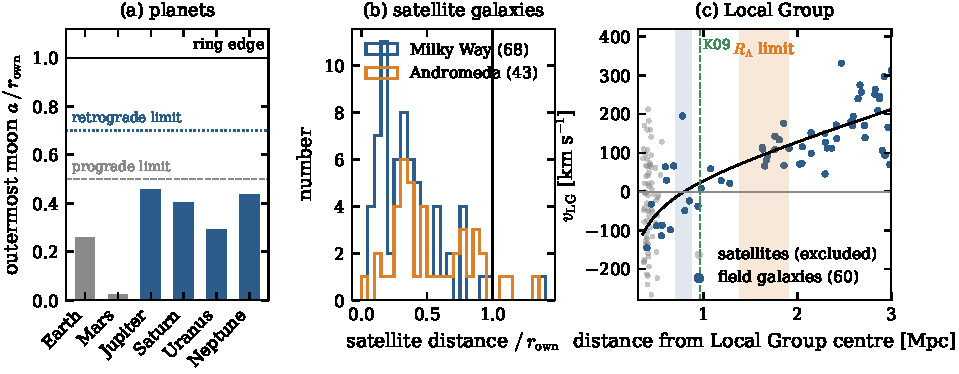
\includegraphics[width=\textwidth]{figures/fig_rings.pdf}
\caption{The balance rule $r_{\rm own}^3=Gm/S$ at three scales. (a) Outermost known moon of six planets as a fraction of $r_{\rm own}$; dashed and dotted lines are the prograde and retrograde stability limits. (b) Distances of 68 Milky Way and 43 M31 satellites as fractions of their hosts' $r_{\rm own}$. (c) Velocities relative to the Local Group centre; blue points are the 60 field galaxies used in the fit (black curve), grey points are excluded satellites. The blue band is the fitted zero-velocity radius, the green dashed line the value of \citet{Karachentsev2009}, and the orange band $R_\Lambda$ for $1.9$--$5\times10^{12}\,M_\odot$.}
\label{fig:rings}
\end{figure}

\subsection{Empty space as the outermost environment}
\label{sec:empty}
The $a_0$ proposal below uses $\Lambda$, so we check it independently with 1,590 Pantheon+ supernovae at $z>0.01$ and their full statistical and systematic covariance \citep{Scolnic2022,Brout2022}. A flat universe with matter and $\Lambda$ gives $\Omega_\Lambda=0.668\pm0.018$, in agreement with the Planck value of 0.685 \citep{Planck2020}. Letting the equation of state vary gives $w=-0.95\pm0.04$, consistent with a constant ($w=-1$). Universes without $\Lambda$ fit worse by $\Delta\chi^2=48$ (empty, coasting), 155 (open, matter only) and 698 (flat, matter only).

\section{The galactic acceleration scale from a presence integral}
\label{sec:a0}

\subsection{Motivation}

The RAR is well described by \citep{McGaugh2016}
\begin{equation}
g_{\rm obs}=\frac{g_{\rm bar}}{1-e^{-\sqrt{g_{\rm bar}/a_0}}}.
\label{eq:rar}
\end{equation}
In the nested sequence of Section~\ref{sec:rings}, empty space is the outermost environment of every system, and its acceleration scale is
\begin{equation}
\aL\equiv c^2\sqrt{\Lambda/3}=cH_0\sqrt{\Omega_\Lambda},
\end{equation}
the surface gravity of the de~Sitter horizon \citep{GibbonsHawking1977}.

\paragraph{Thought experiment: a galaxy alone in empty space.} Place one galaxy in a universe containing only $\Lambda$. Close in, its own pull dominates. Far out, its pull keeps weakening, while empty space supplies a scale $\aL$ that is the same everywhere. The proposal is that the galaxy's dynamics change character where its own pull falls to $\aL$ shared over its ring, $a_0=\aL/k$, with $k$ fixed by how a point source's presence fills a ring. The thought experiment motivates the form; it does not derive it.

\subsection{The factor $k$ from the presence integral}

We define $k$ as the total presence of a point source inside a ring of radius $R$ centred on it, divided by its presence at the edge, in units of $R^n$ for an $n$-dimensional ring:
\begin{equation}
k\equiv\frac{1}{P_{\rm edge}\,R^n}\int_{r<R}P\,dV,\qquad P\propto\frac1r.
\label{eq:k}
\end{equation}
With $dV=S_{n-1}r^{n-1}dr$, where $S_{n-1}$ is the area of the unit sphere in $n$ dimensions (Appendix~\ref{app:k}),
\begin{equation}
k=\frac{S_{n-1}}{n-1}=
\begin{cases}
2\pi/1=2\pi & \text{planar ring } (n=2),\\
4\pi/2=2\pi & \text{spherical ring } (n=3).
\end{cases}
\end{equation}
The factor $\pi$ is not inserted by hand: it comes from the ring being round. The planar and spherical results coincide, so the prediction does not depend on whether a galaxy's ring is taken as a disc or a ball. This equality is special to two and three dimensions; for $n=4$, $k=2\pi^2/3$. Hence
\begin{equation}
a_0=\frac{c^2\sqrt{\Lambda/3}}{2\pi}=\frac{cH_0\sqrt{\Omega_\Lambda}}{2\pi}=
\begin{cases}
0.863\aunit & \text{Planck: } H_0=67.4,\ \Omega_\Lambda=0.685,\\
0.944\aunit & \text{SH0ES: } H_0=73.0,\ \Omega_\Lambda=0.70,
\end{cases}
\label{eq:a0}
\end{equation}
with $H_0$ in km\,s$^{-1}$\,Mpc$^{-1}$ from \citet{Planck2020} and \citet{Riess2022}. Equation~(\ref{eq:a0}) is Milgrom's coincidence \citep{Milgrom1999,Milgrom2016}; what is new is the reason for the $2\pi$. In an earlier version of this work we wrote $k=\pi\langle P\rangle_{\rm in}/P_{\rm edge}$. That form multiplied a two-dimensional factor ($\pi$, the area of the unit disc) by a three-dimensional average and gave $3\pi/2$ for a ball. The consistent integral, Eq.~(\ref{eq:k}), removes that inconsistency and the second value.

Three properties follow:
\begin{enumerate}
\item \textbf{No free parameter.} Given $\Lambda$, Eq.~(\ref{eq:a0}) has one value.
\item \textbf{Universality.} \emph{Thought experiment: the photocopied galaxy.} Build an exact copy of a galaxy ten times larger. Because $P\propto1/r$ has no scale, Eq.~(\ref{eq:k}) is unchanged, and so is $a_0$. The same holds for a heavier copy and, since planar and spherical rings give the same $k$, for a flatter or rounder one. $a_0$ therefore cannot depend on a galaxy's size, mass or visible shape.
\item \textbf{No evolution.} $a_0$ is tied to $\Lambda$, not to the expansion rate, so it is constant in time.
\end{enumerate}

\subsection{Data and fitting}

We use SPARC \citep{Lelli2016}: 3,391 rotation-curve points in 175 galaxies, of which 2,803 points in 164 galaxies have velocity errors below 10\%. For each point $g_{\rm obs}=V_{\rm obs}^2/R$ and $g_{\rm bar}=(V_{\rm gas}^2+\Upsilon_{\rm disk}V_{\rm disk}^2+\Upsilon_{\rm bul}V_{\rm bul}^2)/R$, with fiducial $\Upsilon_{\rm disk}=0.5$ and $\Upsilon_{\rm bul}=0.7$ at 3.6\,$\mu$m \citep{Lelli2016}. When we vary $\Upsilon_{\rm disk}$ we scale the bulge value with it ($\Upsilon_{\rm bul}=1.4\,\Upsilon_{\rm disk}$). We fit $\log g_{\rm obs}$ with Eq.~(\ref{eq:rar}) by
\begin{itemize}
\item minimising the rms of log residuals;
\item minimising $\chi^2$ with velocity-error uncertainties $\sigma=\max[2(\delta V/V)/\ln10,\,0.02]$\,dex;
\item minimising $\chi^2$ with an added intrinsic scatter $\sigma_{\rm int}$ chosen so that $\chi^2/{\rm dof}=1$.
\end{itemize}
Statistical errors come from bootstrapping galaxies. The \emph{gas-rich} subsample contains the 16 galaxies in which gas supplies more than 60\% of $g_{\rm bar}$, on average over points with $g_{\rm bar}<3\aunit$: D631-7, DDO\,154, DDO\,161, DDO\,168, DDO\,170, ESO\,444-G084, F565-V2, KK98-251, NGC\,3109, NGC\,3741, UGC\,00731, UGC\,00891, UGC\,04483, UGC\,05764, UGCA\,442 and UGCA\,444. Per-galaxy fits use galaxies with at least 8 points, excluding fits at the grid boundary (110 galaxies). Disk scale lengths are estimated as $R(V_{\rm disk}^{\rm max})/2.2$. We do not marginalise over distances and inclinations \citep{Li2018}.

\subsection{Results at $z\approx0$}

\paragraph{Gas-rich galaxies.} These are the cleanest test, because stellar mass-to-light ratios barely matter. The best fit is $a_0=0.81\aunit$, and $0.82^{+0.22}_{-0.17}\aunit$ with a galaxy bootstrap. It changes little with $\Upsilon_{\rm disk}$ (0.92, 0.81 and $0.72\aunit$ for 0.25, 0.5 and 0.75) and with the gas threshold (0.78, 0.81 and $0.74\aunit$ for 50\%, 60\% and 70\%, i.e.\ 25, 16 and 11 galaxies). The prediction is consistent: $\Delta\chi^2=+0.1$ (Planck) and $+2.7$ (SH0ES) relative to the best fit, with $\sigma_{\rm int}=0.170$\,dex.

\paragraph{All galaxies.} At the fiducial $\Upsilon_{\rm disk}=0.5$ the rms estimator gives $a_0=1.13\aunit$ (scatter 0.144\,dex), the bootstrap $1.14\pm0.08\aunit$, and the intrinsic-scatter likelihood ($\sigma_{\rm int}=0.134$\,dex) $1.14\aunit$. This is $3.5\sigma$ above the Planck prediction on the bootstrap error alone. The full-sample estimate is, however, strongly degenerate with $\Upsilon$: it falls from 1.47 to $0.90\aunit$ as $\Upsilon_{\rm disk}$ goes from 0.4 to 0.6 (Fig.~\ref{fig:a0}a), and it matches the prediction at $\Upsilon_{\rm disk}=0.62$ (Planck) or 0.58 (SH0ES). At $\Upsilon_{\rm disk}=0.6$ the Planck prediction is within $\Delta\chi^2=+8.4$ of the best fit. Figure~\ref{fig:rar} shows that with $\Upsilon_{\rm disk}=0.62$ the low-acceleration residuals vanish but the highest-acceleration points, where stars dominate, fall about 0.1\,dex below, which suggests the inner disks prefer a lower $\Upsilon$. Points within a galaxy share its distance and inclination errors, so these $\Delta\chi^2$ values overstate significances.

\paragraph{Universality.} Per-galaxy values have median $1.15\aunit$ and scatter 0.26\,dex, much larger than their 0.02\,dex formal errors, as expected from distance, inclination and $\Upsilon$ errors \citep{Li2018}. They show no correlation (Spearman) with
\begin{itemize}
\item disk scale length ($\rho=-0.09$, $p=0.35$), outermost radius ($-0.11$, 0.26) and distance ($-0.07$, 0.49);
\item central surface brightness ($-0.04$, 0.69) and maximum rotation speed ($+0.04$, 0.71);
\item gas fraction ($+0.01$, 0.90) and bulge fraction ($-0.06$, 0.56).
\end{itemize}
Bulge-rich (bulge $>10\%$ of the baryonic mass) and pure-disc galaxies have median $a_0$ of 1.07 and $1.15\aunit$ (Mann--Whitney $p=0.76$); see Fig.~\ref{fig:a0}b. This is the behaviour required by property 2: neither size nor visible shape sets $a_0$. As a contrast, a variant that computes a separate ring factor for each galaxy from its own mass layout predicts $a_0=1.29$--$1.71\aunit$. It fits worse ($\chi^2=53{,}818$ against $49{,}907$ for one universal value, velocity errors only, 113 galaxies), and the galaxies do not follow its predictions ($\rho=0.00$, $p=0.97$). The choice of transition function in Eq.~(\ref{eq:rar}) changes $a_0$ by less than 3\% (``simple'' function: 1.18 and $0.80\aunit$ for all and gas-rich galaxies, against 1.22 and $0.81\aunit$).

\begin{figure}[t]
\centering
\begin{minipage}{0.52\textwidth}\centering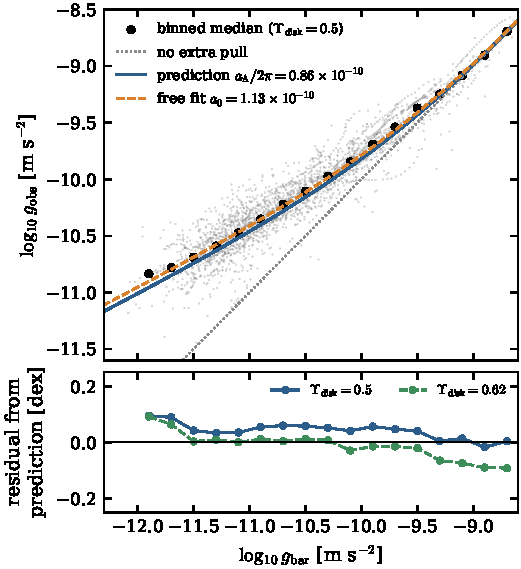
\includegraphics[width=\textwidth]{figures/fig_rar.pdf}\end{minipage}\hfill
\begin{minipage}{0.45\textwidth}
\caption{The radial acceleration relation for 2,803 SPARC points in 164 galaxies at $\Upsilon_{\rm disk}=0.5$, with the predicted $a_0=\aL/2\pi$ (Planck) and the free fit. Black points are binned medians. The lower panel shows median residuals from the prediction at $\Upsilon_{\rm disk}=0.5$ and at $0.62$, where the full-sample fit equals the prediction.}
\label{fig:rar}
\end{minipage}
\end{figure}

\begin{figure}[t]
\centering
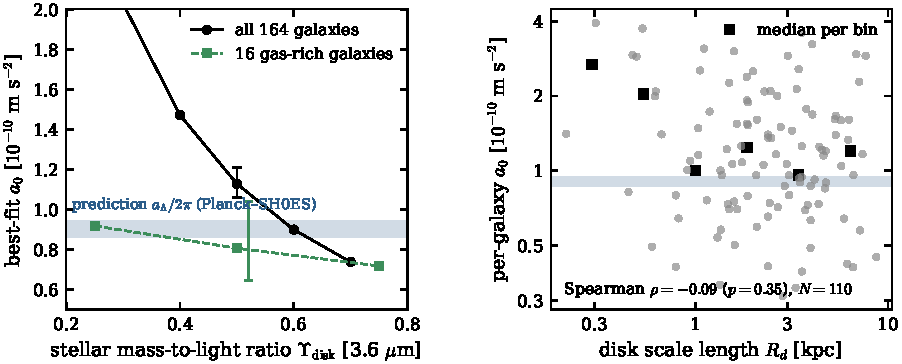
\includegraphics[width=\textwidth]{figures/fig_a0.pdf}
\caption{(a) Best-fit $a_0$ against the assumed stellar mass-to-light ratio, for all 164 galaxies (rms estimator, with bootstrap error at the fiducial value) and for the 16 gas-rich galaxies ($\chi^2$ estimator, with bootstrap error). The band is the prediction $\aL/2\pi$ for Planck to SH0ES parameters. (b) Per-galaxy $a_0$ against disk scale length for 110 galaxies, with binned medians and the prediction band.}
\label{fig:a0}
\end{figure}

\subsection{Does $a_0$ change with redshift?}
\label{sec:time}

Property 3 distinguishes the proposal from relations tied to the expansion rate, $a_0\propto H(z)$, which would make $a_0$ 1.8 times larger at $z=1$ and 3 times larger at $z=2$. We test it with 41 star-forming disks at $z=0.65$--$2.45$ whose redshift, disk effective radius $R_e$, baryonic mass and dark matter fraction $f_{\rm DM}(R_e)$ are tabulated by \citet{Price2021}. If the local RAR holds at $R_e$, then $f_{\rm DM}=\exp(-\sqrt{g_{\rm bar}/a_0})$, so each galaxy gives
\begin{equation}
a_0=\frac{g_{\rm bar}(R_e)}{[\ln f_{\rm DM}(R_e)]^2},
\end{equation}
with $g_{\rm bar}(R_e)$ from half the baryonic mass in a thin exponential disk.

Within the sample, $a_0$ shows no rise with redshift (Fig.~\ref{fig:highz}; Spearman $\rho=+0.08$, $p=0.62$). The median for $z>2$ is 0.89 times that for $z<1.2$ (68\% range 0.78--2.00), where $a_0\propto H(z)$ predicts 2.06. The fitted slope $d\log a_0/d\log H=+0.36$ (68\%: $-0.09$ to $+0.81$) lies between the two hypotheses, so these data cannot yet exclude evolution. The overall level is 1.5--1.9 times the local value for both disk and spherical mass geometries. Because it is the same at every redshift, we attribute it to calibration (baryonic masses from scaling relations, and model-dependent $f_{\rm DM}$) rather than to evolution, but we cannot exclude it.

\begin{figure}[t]
\centering
\begin{minipage}{0.5\textwidth}\centering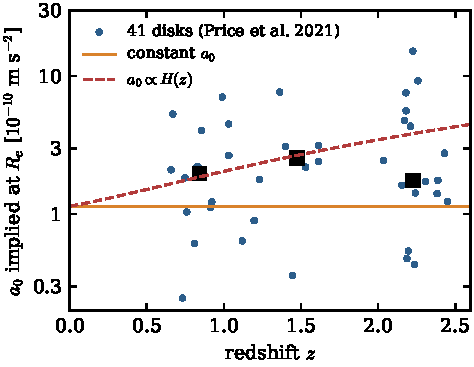
\includegraphics[width=\textwidth]{figures/fig_highz.pdf}\end{minipage}\hfill
\begin{minipage}{0.46\textwidth}
\caption{The $a_0$ implied at the effective radius of 41 disks at $z=0.65$--2.45 \citep{Price2021}, if the local RAR holds there. Squares are medians in three redshift bins. Lines show a constant $a_0$ and $a_0\propto H(z)$, both normalised to the local value. The data show no rise with redshift but a common offset above the local value.}
\label{fig:highz}
\end{minipage}
\end{figure}

\section{Discussion}
\label{sec:discussion}

\subsection{What is new, and what is not}
The presence field, its three readings and the balance rule are reformulations: they reproduce existing physics exactly, and no measurement distinguishes them from the standard description. Their contribution is organisational. The one proposal that could change physics is Eq.~(\ref{eq:a0}) with its derivation, Eq.~(\ref{eq:k}). It links the acceleration at which galaxy dynamics change character to the emptiness that drives cosmic expansion, with the numerical factor fixed by a geometric integral. If confirmed, it would turn a long-noted coincidence into a relation with a reason. It is not yet confirmed.

\subsection{The mass-to-light question and the decisive test}
The gas-rich galaxies agree with the prediction; the full sample agrees only if stellar disks are about 20\% heavier than the fiducial assumption, which the highest-acceleration points do not favour. The decisive test uses gas-dominated galaxies, for which $\Upsilon$ does not matter, with distances accurate to $\sim5\%$ (tip of the red giant branch or Cepheids) and well-measured inclinations. In the low-acceleration regime the inferred $a_0\propto D^{-2}\sin^{-4}i$, so distance and inclination errors dominate the current scatter. Rotation curves of the LITTLE THINGS dwarfs \citep{Iorio2017}, combined with tip-of-the-red-giant-branch distances, are suited to this. A rough baryonic Tully--Fisher estimate for six of them, using catalogue stellar masses, gives 0.84 to $1.12\aunit$ depending on those masses, so it does not yet decide. If such a sample reduces the per-galaxy scatter to about 0.12\,dex, roughly twenty galaxies would measure $a_0$ to about 6\%. That is enough to confirm $0.86$--$0.94\aunit$, or to exclude it if the true value is near 1.15.

\subsection{Relation to modified dynamics and dark matter}
Equation~(\ref{eq:a0}) fixes the value of $a_0$ given $\Lambda$, but not whether the RAR arises from modified dynamics or from dark matter. It does not by itself explain all dynamics: velocity dispersions of 73 Milky Way and M31 satellites, predicted from their luminosities and the RAR before the measured values were loaded, fall short of the measurements by a median factor of 1.45 for the 35 classical satellites and 3.4 for the 38 ultra-faint ones. We therefore remain agnostic about the origin of the RAR and claim only the value of its scale.

\subsection{Limitations}
\begin{itemize}
\item The presence description is equivalent to general relativity in weak fields and makes no new predictions there.
\item Eq.~(\ref{eq:k}) is a definition chosen because it uses presence consistently and gives a shape-independent result. It is not derived from an action, and other plausible definitions would give other factors.
\item The relation was formulated after the SPARC value of $a_0$ and the $2\pi$ coincidence were known. It was revised once, from $\pi\langle P\rangle/P_{\rm edge}$ to Eq.~(\ref{eq:k}), after we found the earlier form mixed dimensions.
\item Our fits fix Eq.~(\ref{eq:rar}) and do not marginalise over distances, inclinations or per-galaxy $\Upsilon$. The high-redshift test relies on published dark matter fractions and simple geometry.
\end{itemize}
The independent tests in Sections~\ref{sec:time} and 5.2 use data not involved in formulating the proposal.

\section{Conclusions}
\begin{enumerate}
\item Weak-field gravity can be read from one scalar, $P=-\Phi/c^2$: its value gives clock rates, its gradient accelerations and its Hessian tides. This reproduces the standard tests (Table~\ref{tab:standard}).
\item The Hill, Jacobi, L1 and $\Lambda$-turnaround radii are one balance condition, $r^3=Gm/S$, with empty space as the final environment. Moons, satellite galaxies, the Local Group and Virgo all sit inside the boundaries it gives, and 1,590 supernovae independently confirm the $\Lambda$ it uses.
\item The total presence of a point source inside a ring, relative to its edge value, equals $2\pi$ for both planar and spherical rings. This gives a parameter-free prediction, $a_0=c^2\sqrt{\Lambda/3}/2\pi=0.86$--$0.94\aunit$, and a reason for the known $2\pi$ coincidence.
\item Gas-rich galaxies agree with it; the full sample agrees if $\Upsilon_{\rm disk}\approx0.6$. $a_0$ is independent of galaxy size, distance, brightness, speed, gas fraction and visible shape, and shows no rise with redshift up to $z\approx2.4$.
\item Gas-dominated galaxies with precise distances can confirm or exclude the prediction.
\end{enumerate}

\section*{Data and code availability}
All numbers and figures come from \texttt{paper\_analysis.py}, \texttt{paper\_additions.py} and the earlier test scripts in the public repository \url{https://github.com/hassan-algo/rings-of-presence}. The repository includes the SPARC rotation curves (CC BY 4.0; \citealt{Lelli2016}) and the Local Volume Database tables (CC0; \citealt{Pace2024}); the Pantheon+ data are downloaded by a script. The high-redshift values are from Table~3 of \citet{Price2021}. Moon orbits are from the JPL Solar System Dynamics planetary satellite mean elements.

\section*{Acknowledgements}
I thank the SPARC team, A.~B.~Pace for the Local Volume Database, the Pantheon+ collaboration and the JPL Solar System Dynamics group for making their data public.
\emph{Use of AI tools:} I used Claude (Anthropic), a large language model, as a research assistant. It helped turn my ideas into equations, wrote and ran the analysis code against the public data, and helped draft the text. Every result was generated by the public scripts and checked against the cited measurements. I take full responsibility for the content of this paper.

\appendix
\section{The presence integral in $n$ dimensions}
\label{app:k}
For $P\propto1/r$ about the centre of an $n$-dimensional ball of radius $R$, with $dV=S_{n-1}r^{n-1}dr$ and $S_{n-1}=2\pi^{n/2}/\Gamma(n/2)$,
\begin{equation}
\frac{1}{P_{\rm edge}R^n}\int_0^R\frac{1}{r}\,S_{n-1}r^{n-1}\,dr=\frac{R}{R^n}\,S_{n-1}\frac{R^{n-1}}{n-1}=\frac{S_{n-1}}{n-1}.
\end{equation}
With $S_1=2\pi$ and $S_2=4\pi$ this gives $2\pi$ for $n=2$ and $n=3$, independent of $R$; $S_3=2\pi^2$ gives $2\pi^2/3$ for $n=4$.

\begin{thebibliography}{99}
\setlength{\itemsep}{1pt}\small\raggedright
\bibitem[Ashby(2003)]{Ashby2003} Ashby N., 2003, Living Rev.\ Relativ., 6, 1. \href{https://doi.org/10.12942/lrr-2003-1}{\texttt{doi:10.12942/lrr-2003-1}}
\bibitem[Bothwell et~al.(2022)]{Bothwell2022} Bothwell T., Kennedy C.~J., Aeppli A., Kedar D., Robinson J.~M., Oelker E., Staron A., Ye J., 2022, Nature, 602, 420. \href{https://doi.org/10.1038/s41586-021-04349-7}{\texttt{doi:10.1038/s41586-021-04349-7}}
\bibitem[Brout et~al.(2022)]{Brout2022} Brout D., et~al., 2022, ApJ, 938, 110. \href{https://arxiv.org/abs/2202.04077}{\texttt{arXiv:2202.04077}}
\bibitem[Eggleton(1983)]{Eggleton1983} Eggleton P.~P., 1983, ApJ, 268, 368. \href{https://doi.org/10.1086/160960}{\texttt{doi:10.1086/160960}}
\bibitem[Famaey \& McGaugh(2012)]{FamaeyMcGaugh2012} Famaey B., McGaugh S.~S., 2012, Living Rev.\ Relativ., 15, 10. \href{https://doi.org/10.12942/lrr-2012-10}{\texttt{doi:10.12942/lrr-2012-10}}
\bibitem[Gibbons \& Hawking(1977)]{GibbonsHawking1977} Gibbons G.~W., Hawking S.~W., 1977, Phys.\ Rev.\ D, 15, 2738. \href{https://doi.org/10.1103/PhysRevD.15.2738}{\texttt{doi:10.1103/PhysRevD.15.2738}}
\bibitem[Hamilton \& Krivov(1997)]{HamiltonKrivov1997} Hamilton D.~P., Krivov A.~V., 1997, Icarus, 128, 241. \href{https://ui.adsabs.harvard.edu/abs/1997Icar..128..241H}{\texttt{ADS:1997Icar..128..241H}}
\bibitem[Iorio et~al.(2017)]{Iorio2017} Iorio G., Fraternali F., Nipoti C., Di Teodoro E., Read J.~I., Battaglia G., 2017, MNRAS, 466, 4159. \href{https://arxiv.org/abs/1611.03865}{\texttt{arXiv:1611.03865}}
\bibitem[Karachentsev et~al.(2009)]{Karachentsev2009} Karachentsev I.~D., Kashibadze O.~G., Makarov D.~I., Tully R.~B., 2009, MNRAS, 393, 1265. \href{https://arxiv.org/abs/0811.4610}{\texttt{arXiv:0811.4610}}
\bibitem[Karachentsev et~al.(2014)]{Karachentsev2014} Karachentsev I.~D., Tully R.~B., Wu P.-F., Shaya E.~J., Dolphin A.~E., 2014, ApJ, 782, 4. \href{https://arxiv.org/abs/1312.6769}{\texttt{arXiv:1312.6769}}
\bibitem[Keller \& Wadsley(2017)]{KellerWadsley2017} Keller B.~W., Wadsley J.~W., 2017, ApJ, 835, L17. \href{https://doi.org/10.3847/2041-8213/835/1/L17}{\texttt{doi:10.3847/2041-8213/835/1/L17}}
\bibitem[King(1962)]{King1962} King I., 1962, AJ, 67, 471. \href{https://doi.org/10.1086/108756}{\texttt{doi:10.1086/108756}}
\bibitem[Lelli et~al.(2016)]{Lelli2016} Lelli F., McGaugh S.~S., Schombert J.~M., 2016, AJ, 152, 157. \href{https://doi.org/10.3847/0004-6256/152/6/157}{\texttt{doi:10.3847/0004-6256/152/6/157}}
\bibitem[Lelli et~al.(2017)]{Lelli2017} Lelli F., McGaugh S.~S., Schombert J.~M., Pawlowski M.~S., 2017, ApJ, 836, 152. \href{https://doi.org/10.3847/1538-4357/836/2/152}{\texttt{doi:10.3847/1538-4357/836/2/152}}
\bibitem[Li et~al.(2018)]{Li2018} Li P., Lelli F., McGaugh S., Schombert J., 2018, A\&A, 615, A3. \href{https://doi.org/10.1051/0004-6361/201732547}{\texttt{doi:10.1051/0004-6361/201732547}}
\bibitem[Ludlow et~al.(2017)]{Ludlow2017} Ludlow A.~D., et~al., 2017, Phys.\ Rev.\ Lett., 118, 161103. \href{https://doi.org/10.1103/PhysRevLett.118.161103}{\texttt{doi:10.1103/PhysRevLett.118.161103}}
\bibitem[McGaugh et~al.(2016)]{McGaugh2016} McGaugh S.~S., Lelli F., Schombert J.~M., 2016, Phys.\ Rev.\ Lett., 117, 201101. \href{https://doi.org/10.1103/PhysRevLett.117.201101}{\texttt{doi:10.1103/PhysRevLett.117.201101}}
\bibitem[Milgrom(1983)]{Milgrom1983} Milgrom M., 1983, ApJ, 270, 365. \href{https://doi.org/10.1086/161130}{\texttt{doi:10.1086/161130}}
\bibitem[Milgrom(1999)]{Milgrom1999} Milgrom M., 1999, Phys.\ Lett.\ A, 253, 273. \href{https://doi.org/10.1016/S0375-9601(99)00077-8}{\texttt{doi:10.1016/S0375-9601(99)00077-8}}
\bibitem[Milgrom(2016)]{Milgrom2016} Milgrom M., 2016. \href{https://arxiv.org/abs/1605.07458}{\texttt{arXiv:1605.07458}}
\bibitem[M\"uller et~al.(2023)]{Muller2023} M\"uller J., Biskupek L., Singh V., Zhang M., 2023, Using LLR data for testing general relativity with focus on the equivalence principle, ILRS Workshop 2023. \href{https://ilrs.cddis.eosdis.nasa.gov/lw23/docs/presentations/S03/S03-03_LLR-ILRS-WS2023JM_Jurgen_presentation.pdf}{\texttt{presentation (PDF)}}
\bibitem[Murray \& Dermott(1999)]{MurrayDermott1999} Murray C.~D., Dermott S.~F., 1999, Solar System Dynamics. Cambridge Univ.\ Press, Cambridge. \href{https://doi.org/10.1017/CBO9781139174817}{\texttt{doi:10.1017/CBO9781139174817}}
\bibitem[Pace(2024)]{Pace2024} Pace A.~B., 2024. \href{https://arxiv.org/abs/2411.07424}{\texttt{arXiv:2411.07424}}
\bibitem[Pavlidou \& Tomaras(2014)]{PavlidouTomaras2014} Pavlidou V., Tomaras T.~N., 2014, J.\ Cosmol.\ Astropart.\ Phys., 09, 020. \href{https://doi.org/10.1088/1475-7516/2014/09/020}{\texttt{doi:10.1088/1475-7516/2014/09/020}}
\bibitem[Planck Collaboration(2020)]{Planck2020} Planck Collaboration, 2020, A\&A, 641, A6. \href{https://doi.org/10.1051/0004-6361/201833910}{\texttt{doi:10.1051/0004-6361/201833910}}
\bibitem[Price et~al.(2021)]{Price2021} Price S.~H., Shimizu T.~T., Genzel R., et~al., 2021, ApJ, 922, 143. \href{https://arxiv.org/abs/2109.02659}{\texttt{arXiv:2109.02659}}
\bibitem[Riess et~al.(2022)]{Riess2022} Riess A.~G., et~al., 2022, ApJ, 934, L7. \href{https://doi.org/10.3847/2041-8213/ac5c5b}{\texttt{doi:10.3847/2041-8213/ac5c5b}}
\bibitem[Scolnic et~al.(2022)]{Scolnic2022} Scolnic D., et~al., 2022, ApJ, 938, 113. \href{https://arxiv.org/abs/2112.03863}{\texttt{arXiv:2112.03863}}
\bibitem[Tolman et~al.(1931)]{Tolman1931} Tolman R.~C., Ehrenfest P., Podolsky B., 1931, Phys.\ Rev., 37, 602. \href{https://doi.org/10.1103/PhysRev.37.602}{\texttt{doi:10.1103/PhysRev.37.602}}
\bibitem[Weisberg \& Huang(2016)]{WeisbergHuang2016} Weisberg J.~M., Huang Y., 2016, ApJ, 829, 55. \href{https://doi.org/10.3847/0004-637X/829/1/55}{\texttt{doi:10.3847/0004-637X/829/1/55}}
\bibitem[Will(2014)]{Will2014} Will C.~M., 2014, Living Rev.\ Relativ., 17, 4. \href{https://doi.org/10.12942/lrr-2014-4}{\texttt{doi:10.12942/lrr-2014-4}}
\end{thebibliography}

\end{document}
